\section{Trigger efficiency}
\label{sec:trgEff}


\begin{figure}[tbh]
\begin{center}
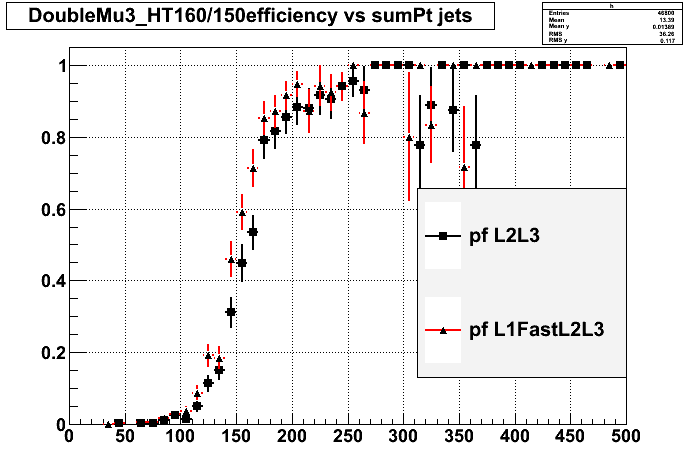
\includegraphics[width=0.6\linewidth]{plots/httrig.png}
\caption{\label{fig:httrig}\protect Efficiency for the dimuon-\Ht\ trigger as a function of the offline \Ht. 
The efficiencies with respect to \Ht\ constructed from pfjets with L2L3 vs. L1FastL2L3 corrections
are shown (we use the latter).
{\bf WILL UPDATE WITH PRETTIER PICTURE COMPARING $ee$, $\mu\mu$, $e\mu$ TRIGGER EFFICIENCIES.}
}
\end{center}
\end{figure}

For the high \pt dilepton triggers, the efficiencies have been measured to be approximately
100\% (DoubleEle), 90\% (DoubleMu), and 95\% (Mu-Ele)~\cite{ref:HWW}. 
In the following, unless otherwise specified we weight the $ee$, $\mu\mu$ and $e\mu$ MC events 
by these efficiencies. We do not apply any efficiency correction for the hadronic 
part of the dilepton-\Ht\ triggers. We have verified that the efficiencies for these triggers
with respect to an offline selection of \Ht\ $>$ 200 GeV is high ($\sim$90--95\%), 
as shown in Fig.~\ref{fig:httrig}.



